\documentclass{standalone}
\usepackage[margin=1in]{geometry}
\usepackage[hang,small,bf]{caption}
\usepackage{tikz}
\usepackage{braket}
\usetikzlibrary{backgrounds,shadows.blur,fit,decorations.pathreplacing,shapes}

\begin{document}
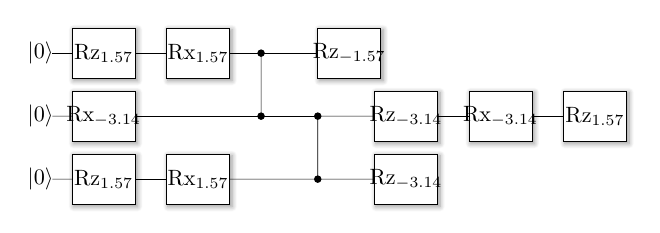
\begin{tikzpicture}[scale=0.8, transform shape]

\tikzstyle{basicshadow}=[blur shadow={shadow blur steps=8, shadow xshift=0.7pt, shadow yshift=-0.7pt, shadow scale=1.02}]\tikzstyle{basic}=[draw,fill=white,basicshadow]
\tikzstyle{operator}=[basic,minimum size=1.5em]
\tikzstyle{phase}=[fill=black,shape=circle,minimum size=0.1cm,inner sep=0pt,outer sep=0pt,draw=black]
\tikzstyle{none}=[inner sep=0pt,outer sep=-.5pt,minimum height=0.5cm+1pt]
\tikzstyle{measure}=[operator,inner sep=0pt,minimum height=0.5cm, minimum width=0.75cm]
\tikzstyle{xstyle}=[circle,basic,minimum height=0.35cm,minimum width=0.35cm,inner sep=-1pt,very thin]
\tikzset{
shadowed/.style={preaction={transform canvas={shift={(0.5pt,-0.5pt)}}, draw=gray, opacity=0.4}},
}
\tikzstyle{swapstyle}=[inner sep=-1pt, outer sep=-1pt, minimum width=0pt]
\tikzstyle{edgestyle}=[very thin]

\node[none] (line0_gate0) at (0.1,-0) {$\Ket{0}$};
\node[none] (line0_gate1) at (0.6000000000000001,-0) {};
\node[none,minimum height=0.8cm,outer sep=0] (line0_gate2) at (1.1,-0) {};
\node[none] (line0_gate3) at (1.6,-0) {};
\draw[operator,edgestyle,outer sep=1.0cm] ([yshift=0.4cm]line0_gate1) rectangle ([yshift=-0.4cm]line0_gate3) node[pos=.5] {Rz$_{1.57}$};
\draw (line0_gate0) edge[edgestyle] (line0_gate1);
\node[none] (line0_gate4) at (2.1,-0) {};
\node[none,minimum height=0.8cm,outer sep=0] (line0_gate5) at (2.6,-0) {};
\node[none] (line0_gate6) at (3.1,-0) {};
\draw[operator,edgestyle,outer sep=1.0cm] ([yshift=0.4cm]line0_gate4) rectangle ([yshift=-0.4cm]line0_gate6) node[pos=.5] {Rx$_{1.57}$};
\draw (line0_gate3) edge[edgestyle] (line0_gate4);
\node[none] (line1_gate0) at (0.1,-1) {$\Ket{0}$};
\node[none] (line1_gate1) at (0.6000000000000001,-1) {};
\node[none,minimum height=0.8cm,outer sep=0] (line1_gate2) at (1.1,-1) {};
\node[none] (line1_gate3) at (1.6,-1) {};
\draw[operator,edgestyle,outer sep=1.0cm] ([yshift=0.4cm]line1_gate1) rectangle ([yshift=-0.4cm]line1_gate3) node[pos=.5] {Rx$_{-3.14}$};
\draw (line1_gate0) edge[edgestyle] (line1_gate1);
\node[phase] (line0_gate7) at (3.6,-0) {};
\node[phase] (line1_gate4) at (3.6,-1) {};
\draw (line1_gate4) edge[edgestyle] (line0_gate7);
\draw (line0_gate6) edge[edgestyle] (line0_gate7);
\draw (line1_gate3) edge[edgestyle] (line1_gate4);
\node[none] (line0_gate8) at (4.500000000000001,-0) {};
\node[none,minimum height=0.8cm,outer sep=0] (line0_gate9) at (5.000000000000001,-0) {};
\node[none] (line0_gate10) at (5.500000000000001,-0) {};
\draw[operator,edgestyle,outer sep=1.0cm] ([yshift=0.4cm]line0_gate8) rectangle ([yshift=-0.4cm]line0_gate10) node[pos=.5] {Rz$_{-1.57}$};
\draw (line0_gate7) edge[edgestyle] (line0_gate8);
\node[none] (line2_gate0) at (0.1,-2) {$\Ket{0}$};
\node[none] (line2_gate1) at (0.6000000000000001,-2) {};
\node[none,minimum height=0.8cm,outer sep=0] (line2_gate2) at (1.1,-2) {};
\node[none] (line2_gate3) at (1.6,-2) {};
\draw[operator,edgestyle,outer sep=1.0cm] ([yshift=0.4cm]line2_gate1) rectangle ([yshift=-0.4cm]line2_gate3) node[pos=.5] {Rz$_{1.57}$};
\draw (line2_gate0) edge[edgestyle] (line2_gate1);
\node[none] (line2_gate4) at (2.1,-2) {};
\node[none,minimum height=0.8cm,outer sep=0] (line2_gate5) at (2.6,-2) {};
\node[none] (line2_gate6) at (3.1,-2) {};
\draw[operator,edgestyle,outer sep=1.0cm] ([yshift=0.4cm]line2_gate4) rectangle ([yshift=-0.4cm]line2_gate6) node[pos=.5] {Rx$_{1.57}$};
\draw (line2_gate3) edge[edgestyle] (line2_gate4);
\node[phase] (line2_gate7) at (4.500000000000001,-2) {};
\node[phase] (line1_gate5) at (4.500000000000001,-1) {};
\draw (line1_gate5) edge[edgestyle] (line2_gate7);
\draw (line2_gate6) edge[edgestyle] (line2_gate7);
\draw (line1_gate4) edge[edgestyle] (line1_gate5);
\node[none] (line1_gate6) at (5.400000000000001,-1) {};
\node[none,minimum height=0.8cm,outer sep=0] (line1_gate7) at (5.900000000000001,-1) {};
\node[none] (line1_gate8) at (6.400000000000001,-1) {};
\draw[operator,edgestyle,outer sep=1.0cm] ([yshift=0.4cm]line1_gate6) rectangle ([yshift=-0.4cm]line1_gate8) node[pos=.5] {Rz$_{-3.14}$};
\draw (line1_gate5) edge[edgestyle] (line1_gate6);
\node[none] (line1_gate9) at (6.900000000000001,-1) {};
\node[none,minimum height=0.8cm,outer sep=0] (line1_gate10) at (7.400000000000001,-1) {};
\node[none] (line1_gate11) at (7.900000000000001,-1) {};
\draw[operator,edgestyle,outer sep=1.0cm] ([yshift=0.4cm]line1_gate9) rectangle ([yshift=-0.4cm]line1_gate11) node[pos=.5] {Rx$_{-3.14}$};
\draw (line1_gate8) edge[edgestyle] (line1_gate9);
\node[none] (line1_gate12) at (8.4,-1) {};
\node[none,minimum height=0.8cm,outer sep=0] (line1_gate13) at (8.9,-1) {};
\node[none] (line1_gate14) at (9.4,-1) {};
\draw[operator,edgestyle,outer sep=1.0cm] ([yshift=0.4cm]line1_gate12) rectangle ([yshift=-0.4cm]line1_gate14) node[pos=.5] {Rz$_{1.57}$};
\draw (line1_gate11) edge[edgestyle] (line1_gate12);
\node[none] (line2_gate8) at (5.400000000000001,-2) {};
\node[none,minimum height=0.8cm,outer sep=0] (line2_gate9) at (5.900000000000001,-2) {};
\node[none] (line2_gate10) at (6.400000000000001,-2) {};
\draw[operator,edgestyle,outer sep=1.0cm] ([yshift=0.4cm]line2_gate8) rectangle ([yshift=-0.4cm]line2_gate10) node[pos=.5] {Rz$_{-3.14}$};
\draw (line2_gate7) edge[edgestyle] (line2_gate8);

\end{tikzpicture}
\end{document}
